\documentclass{standalone}

\usepackage{tikz}
\usetikzlibrary{positioning}
\usetikzlibrary{er}

\begin{document}
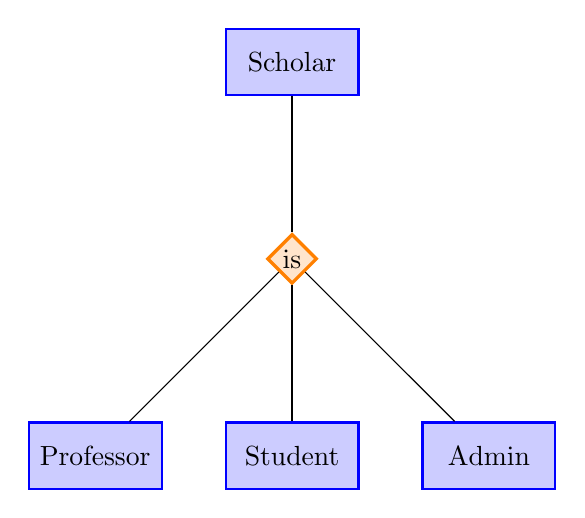
\begin{tikzpicture}
    [
    node distance=2.5cm and 2.5cm,
    on grid,
    every node/.style={draw,rectangle},
    every entity/.style={fill=blue!20, draw=blue, thick},
    every relationship/.style={fill=orange!20, draw=orange, very thick},
    every attribute/.style={fill=gray!20, draw=gray, thick},
    every pin edge/.style=draw,
    ]

    \node[entity] (scholar) {Scholar};
    
    \node[relationship, below = of scholar] (is_rel) {is} edge (scholar)
    child {node [entity, below = of is_rel] (student) {Student}}
    child {node [entity, below right = of is_rel] (admin) {Admin}}
    child {node [entity, below left = of is_rel] (professor) {Professor}};
\end{tikzpicture}
\end{document}
